\documentclass[10pt,xcolor=pdflatex]{beamer}
\usepackage{newcent}
\usepackage[utf8]{inputenc}
\usepackage[czech]{babel}
\usepackage{hyperref}
\usepackage{fancyvrb}
\usepackage{verbatim}
\usepackage{multirow}
\usetheme{FIT}

%%%%%%%%%%%%%%%%%%%%%%%%%%%%%%%%%%%%%%%%%%%%%%%%%%%%%%%%%%%%%%%%%%
\title[]{Určení typu a směru zbraně v obrazové scéně}

\author[]{Róbert Kolcún}

\institute[]{Vysoké Učení Technické v Brně, Fakulta Informačních Technológií\\
Bo\v{z}et\v{e}chova 1/2. 612 66 Brno - Kr\'alovo Pole\\
xkolcu00@fit.vutbr.cz}

%\date{January 1, 2016}
\date{\today}
%\date{} % bez data

%%%%%%%%%%%%%%%%%%%%%%%%%%%%%%%%%%%%%%%%%%%%%%%%%%%%%%%%%%%%%%%%%%

\begin{document}
% Title page
\frame[plain]{\titlepage}


\begin{comment}
    % Frame
    \begin{frame}\frametitle{Frame Title}
        Example \emph{content}.
    \end{frame}
\end{comment}


% Frame
\begin{frame}\frametitle{Cieľ práce}
    \begin{itemize}
        \item Klasifikácia zbraní do dvoch kategórií.
        \item Určenie náklonu zbrane v troch osách.
    \end{itemize}

    \begin{figure}[H]
        \centering
        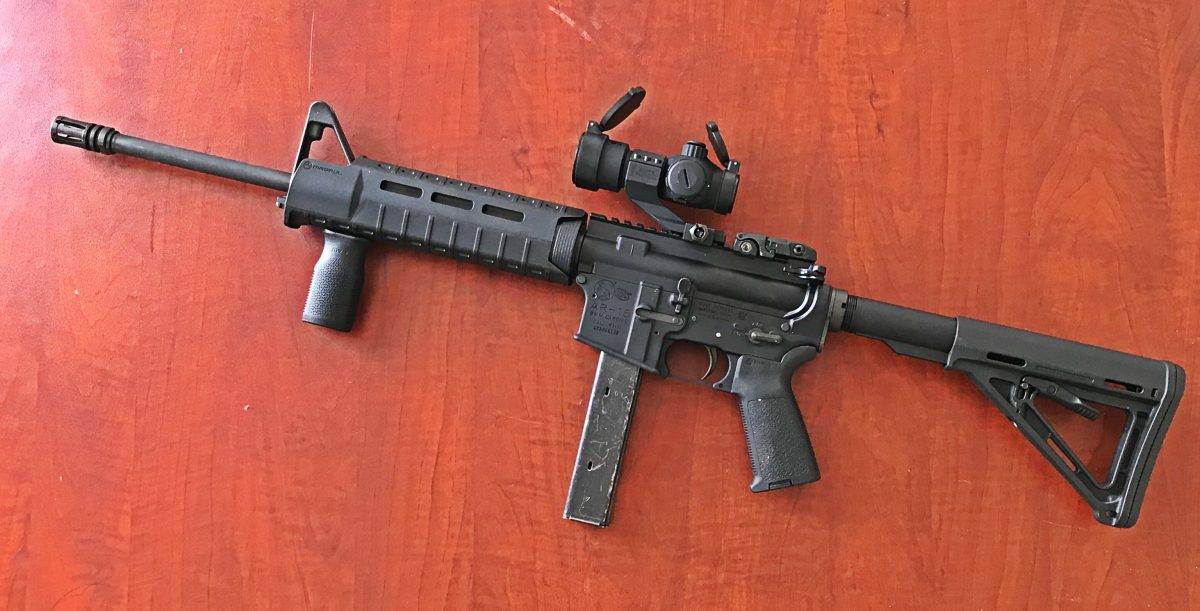
\includegraphics[width=0.5\textwidth]{img/long-weapon}
        \qquad
        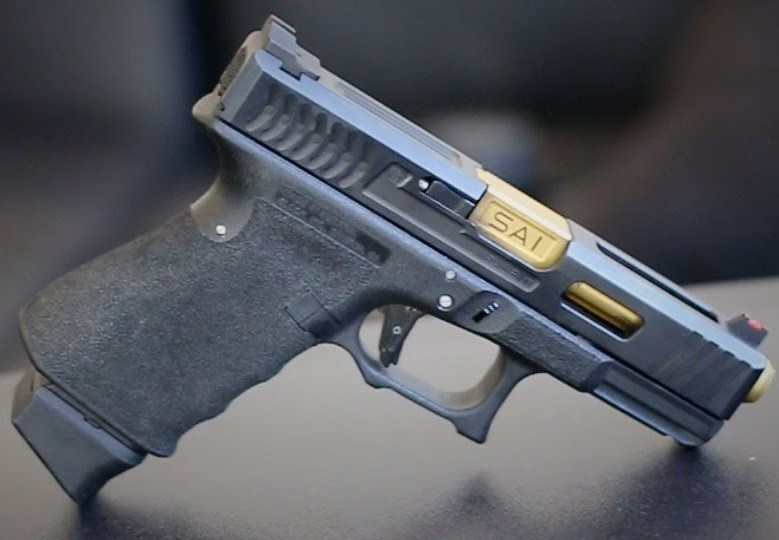
\includegraphics[width=0.4\textwidth]{img/short-weapon}
        \caption{Príklad vstupných dát.}
    \end{figure}

\end{frame}


% Frame
\begin{frame}\frametitle{Návrhovaný postup}
    \begin{itemize}
        \item Predspracovanie obrazu
        \begin{itemize}
            \item Hoghova tranformácia obrazu

            \begin{figure}[H]
                \centering
                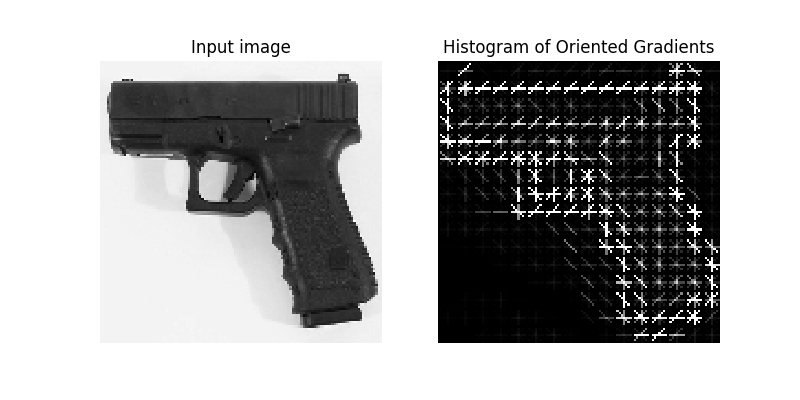
\includegraphics[width=0.55\textwidth]{img/hog}
                \caption{Príklad Hoghovej transformácie vstupných dát.}
            \end{figure}

            \item Augmentácia dát

            \begin{figure}[H]
                \centering
                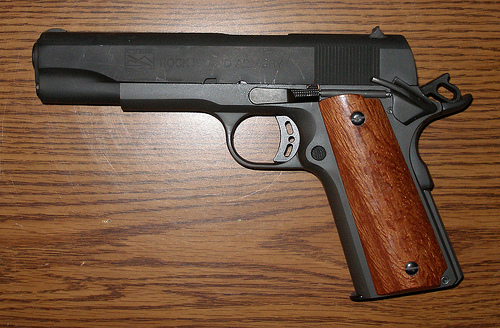
\includegraphics[width=0.3\textwidth]{img/weapon}
                \qquad
                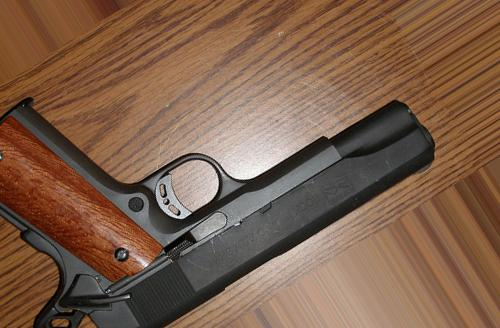
\includegraphics[width=0.30\textwidth]{img/weapon-augmented}
                \caption{Originálny obrázok(vľavo), augmentovaný obrázok(vpravo).}
            \end{figure}
        \end{itemize}
    \end{itemize}
\end{frame}

% Frame
\begin{frame}\frametitle{Klasifikácia}
    \begin{itemize}
        \item Klasifikácia zbrane do dvoch kategórií
        \begin{itemize}
            \item krátke a dlhé
            \vspace{0.2cm}
            \item Klasický prístup - SVM, K-Nearest-Neigbour
            \item Konvolučné neurónové siete - 2 architektúry (AlexNetLike, VGGLike)
        \end{itemize}

        \vspace{0.1cm}

        \item Určenie náklonu zbrane
        \begin{itemize}
            \item Klasifikácia do 72 kategórií po 5 stupňov.
            \item Tri modely, jeden pre každú z troch osí.
            \vspace{0.2cm}
            \item Konvolučné neurónové siete - 2 architektúry (AlexNetLike, VGGLike)
        \end{itemize}

        \vspace{0.3cm}

        \item Použité knižnice
        \begin{itemize}
            \item scikit-image, Keras - predspracovanie obrazu
            \item scikit-learn, Keras - algoritmy strojového učenia
        \end{itemize}

    \end{itemize}
\end{frame}
\begin{comment}
    - pre klasicky pristup bola pouzita Hoghova transformacia
    - pre CNN bola pouzita augmentacia dat pre zvacsenie mnozstva vstupnych datasetov
    - vsetky postupy boli implementovane a nasledne porovnane
\end{comment}

% Frame
\begin{frame}\frametitle{Výsledky}
    \begin{table}
        \begin{tabular}{ l | c | c }
            \textbf{Klasifikácia}   & \textbf{Model}                    & \textbf{Presnosť}   \\
            \hline \hline
            \textit{Krátke/Dlhé}    &                                   & {83,14\%}           \\
            \hline
            \textit{Pitch}          &                                   & {85,14\%}           \\
            \textit{Roll}           &                                   & {91,02\%}           \\
            \textit{Yaw}            & \multirow{-4}{*}{AlexNetLike}     & {49,71\%}
        \end{tabular}
        \caption{Výsledna presnosť modelov.}
    \end{table}

    \begin{figure}[H]
        \centering
        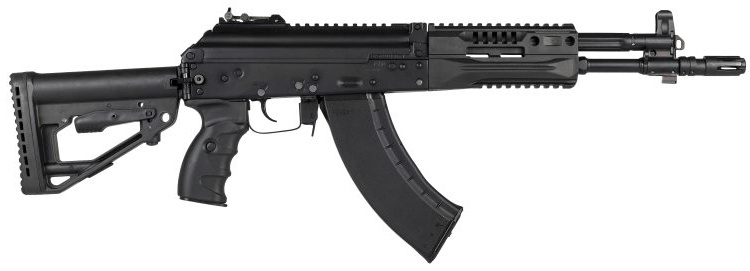
\includegraphics[width=0.6\textwidth]{img/prediction-weapon}
        \caption{Obrázok zbrane pre príklad výstupu klasfikácie nižšie.}
    \end{figure}

    \begin{figure}[H]
        \centering
        
\includegraphics[width=1\textwidth]{img/result-prediction}
    \end{figure}

\end{frame}

% Last page
\bluepage{Ďakujem za pozornosť.}


% Frame
\begin{frame}\frametitle{Otázky oponenta}
    \begin{itemize}
        \item \dots
        \item \dots
    \end{itemize}
\end{frame}


\end{document}
